\documentclass[tikz,border=10pt]{standalone}
\usepackage[T1]{fontenc}
\usepackage{lmodern,amsmath,amssymb}
\usetikzlibrary{arrows.meta,positioning}
\definecolor{ink}{HTML}{183444}
\definecolor{blue}{HTML}{1B6780}
\definecolor{amber}{HTML}{AD601A}
\begin{document}
\hyphenpenalty=10000\exhyphenpenalty=10000
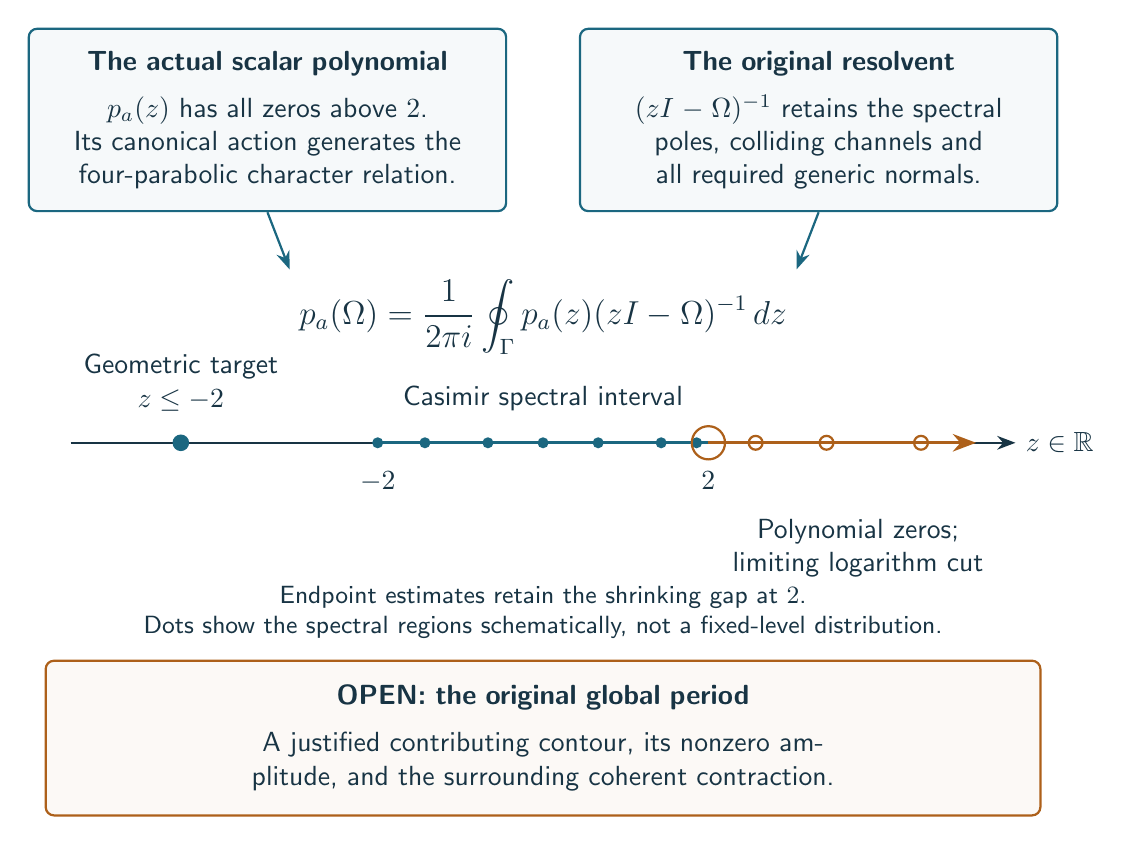
\begin{tikzpicture}[font=\sffamily,text=ink,>=Stealth,
 box/.style={draw=blue,thick,rounded corners=3pt,fill=blue!4,text width=5.5cm,minimum height=2.1cm,align=center,inner sep=8pt}]
 \node[box] (p) at (0,0) {\textbf{The actual scalar polynomial}\\[5pt]
 $p_a(z)$ has all zeros above $2$.\\
 Its canonical action generates the\\four-parabolic character relation.};
 \node[box] (r) at (7,0) {\textbf{The original resolvent}\\[5pt]
 $(zI-\Omega)^{-1}$ retains the spectral\\poles, colliding channels and\\all required generic normals.};
 \node[align=center,font=\sffamily\large] (i) at (3.5,-2.5)
 {$\displaystyle p_a(\Omega)=\frac{1}{2\pi i}\oint_\Gamma p_a(z)(zI-\Omega)^{-1}\,dz$};
 \draw[->,thick,blue] (p.south)--(i.north west);
 \draw[->,thick,blue] (r.south)--(i.north east);
 \draw[->,thick,ink] (-2.5,-4.1)--(9.5,-4.1) node[right] {$z\in\mathbb R$};
 \draw[very thick,blue] (1.4,-4.1)--(5.6,-4.1);
 \foreach \x in {1.4,2,2.8,3.5,4.2,5,5.45} {\fill[blue] (\x,-4.1) circle (2pt);}
 \draw[very thick,amber,->] (5.6,-4.1)--(9,-4.1);
 \foreach \x in {6.2,7.1,8.3} {\draw[amber,thick] (\x,-4.1) circle (2.5pt);}
 \node[below=7pt] at (1.4,-4.1) {$-2$};
 \node[below=7pt] at (5.6,-4.1) {$2$};
 \node[above=8pt,align=center] at (3.5,-4.1) {Casimir spectral interval};
 \node[below=24pt,align=center] at (7.5,-4.1) {Polynomial zeros;\\limiting logarithm cut};
 \fill[blue] (-1.1,-4.1) circle (3pt);
 \node[above=8pt,align=center] at (-1.1,-4.1) {Geometric target\\$z\leq-2$};
 \draw[amber,thick] (5.6,-4.1) circle (6pt);
 \node[font=\sffamily\small,align=center,text width=12cm] at (3.5,-6.25)
 {Endpoint estimates retain the shrinking gap at $2$.\\Dots show the spectral regions schematically, not a fixed-level distribution.};
 \node[draw=amber,thick,rounded corners=3pt,fill=amber!4,text width=12cm,align=center,inner sep=9pt] at (3.5,-7.85)
 {\textbf{OPEN: the original global period}\\[5pt]
 A justified contributing contour, its nonzero amplitude, and the surrounding coherent contraction.};
\end{tikzpicture}
\end{document}
